%SourceDoc ../YourName-Dissertation.tex
\vspace*{-80mm}
\chapter{Isokinetic Step Advection} \label{chapter4:Isokinetic_Step_Advection}
 
	\section{Problem Setup} \label{Verification:Advection}
    
    A tube with no gravity acting in the direction of fluid flow has an initial
    condition of $U_{1},\rho_{1},h_{1},P_{1},\dot{m}_{1}$ everywhere except at the 
    starting position that has an intitial conditions of $h_{2},\rho_{2},\dot{m}_{2}$. 
    When the time step for the calcuation is taken be exactly equal to the CFL
    number as seen in equation \ref{eq:CFL}, the inlet conditions should advect
    through the rest of the system in the form of a square wave. This is a
    unique situation where the CFL can be held constant throughout the
    simulation, and where the spatial and temporal trucation error can cancel
    each other out at $CFL=1$. When the CFL is less than 1, numerical
    diffusion occurs based on the truncation terms produced by the modified
    equation analysis.
    
    \begin{equation}
    	\label{eq:CFL}
    	CFL = \frac{\Delta t  U_{0} }{\Delta x}
    \end{equation}
    
    \begin{figure}[!h]
    	\centering
    	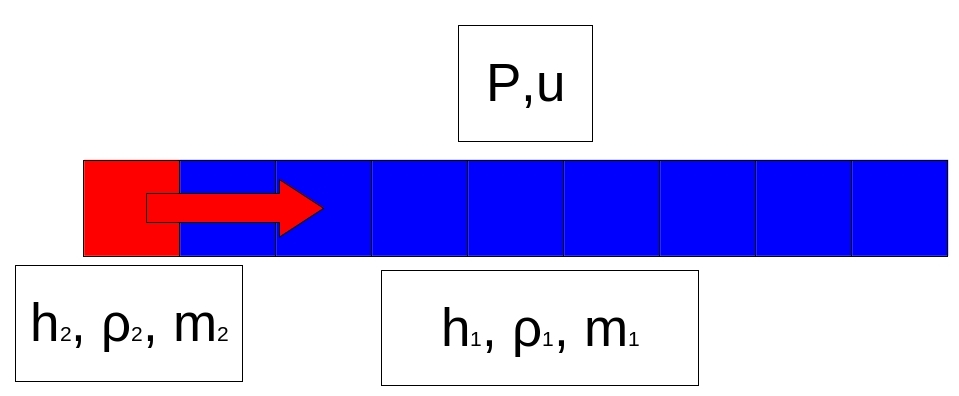
\includegraphics[width=0.65\textwidth]{images/Verification_Problem1_advection}
    	\label{fig:Verification_1}
    	\caption{Setup for the isokinetic advection problem}
    \end{figure}
    
    The problem was set up using the parameters given in table
    \ref{table:Advection_Params}. Initial temperature, density, and mass flow
    rate of the sysmte differs from the inlet temperature, density, and mass
    flow rate. The pressure and velocity of the system remains constant. The
    transient runs until the center of the advected wave reaches the end of the
    tube at roughly 60 seconds. The value of the parameters are more or less
    arbitrary, but approximate a single channel about the length of a fuel
    assembly undergoing a 10 C temperature difference. The water is close to
    standard temperature and pressure. 
    
    \begin{table}[!h]
    	\center
    	\label{table:Advection_Params}
    	\caption{Input Parameters for Isokinetic Advection}
    	\begin{tabular}{|c|c|c|}
    		\hline
	    	Length 	  				&  3.00		& m 		\\ \hline 
	    	Channel Area			&  0.0001	& $m^{2}$	\\ \hline
	    	Wetted Perimeter		&  0.040	& m			\\ \hline
	    	Pressure  				&  1.00		& bar		\\ \hline
	    	Initial Temperature		&  40.00	& C			\\ \hline
	    	Inlet Temperature		&  30.00 	& C			\\ \hline
	    	Inlet Mass Flow Rate 	&  0.005	& kg/s		\\ \hline 
	    	Inlet Density			&  992.61	& kg/$m^{3}$\\ \hline
	    	Velocity				&  0.050372	& m/s		\\ \hline
    	\end{tabular}
    \end{table}
    
    \section{Density Advection and Error}
    
    Figure \ref{fig:enthalpy_wave} compares the analytical and numerical
    advection of density through the domain for a CFL number of 0.500. The
    higher density in the colder region is on the left, and the lower density of
    the warmer region is on the right. The red line on the right of the figure
    depicts the truncation error at the current time step. The truncation error
    occurs around the original dicontinuity as it advects through the solution.
    As the discontinuity propogates it becomes more diffuse spatially. Once it
    reaches the outlet the discontiuty leaves the domain and the overall error
    drops to nearly zero. For this problem, the truncation error can be shown to
    be a direct function of the CFL number and can be reduced to nearly zero
    throughout the simulation. This simplified problem with an exact solution is
    used for code verification.
    
    \begin{figure}[!h]
    	\centering
   		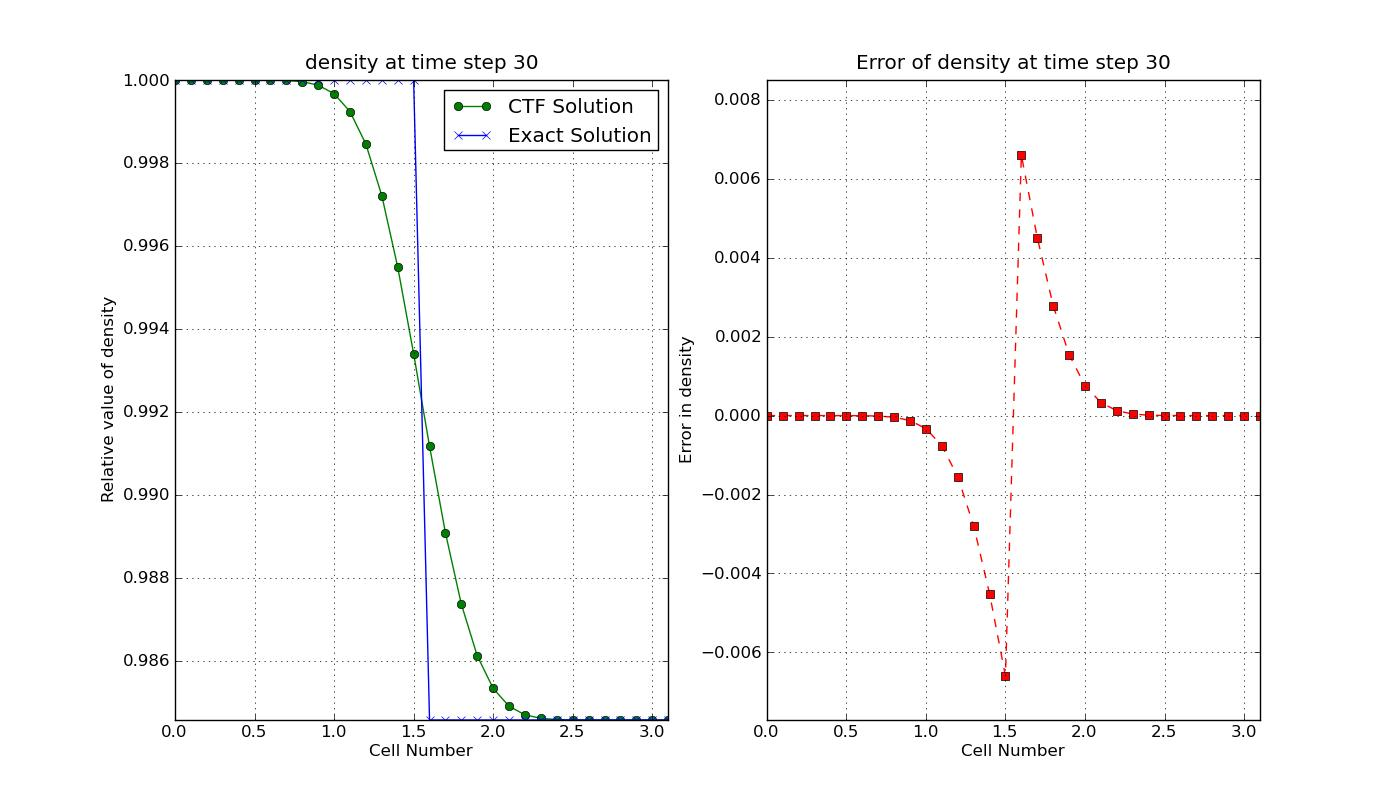
\includegraphics[width=0.85\textwidth]{images/linear_CTF_CFL_0.500/tmp/plot_density_0030}
    	\caption{Comparison of density advection to analytical solution}
    	\label{fig:enthalpy_wave}
    \end{figure}
    
    \section{Modified Equation Analysis}
    
    For this isokinetic problem, the original mass balance equation can be re-written to 
    look like equation \ref{eq:isokinetic_start}. Using upwinding, the finite difference
    can be written to look like equation \ref{eq:mass_isok_fd}. A second order Taylor 
    series approximation can be used for $\rho_{i}^{n+1}$ and $\rho_{i-1}^{n}$ as shown 
    in equations \ref{eq:rho_taylor_series_time} and \ref{eq:rho_taylor_series_space} 
    respectively. The higher order terms ($O(\Delta x^{2},\Delta t^{2} )$) are
    not taken into account for this approximation. The Taylor series
    approximations can then be substituted into \ref{eq:mass_isok_fd} to yield
    \ref{eq:MEA_start}. This is the beginning of the modified equation analysis.
    The goal will be to isolate the original PDE and define the truncation error.
    
    \begin{equation}
    	\label{eq:isokinetic_start}
    	\frac{\partial \rho}{\partial t} + U_{0} \frac{\partial \rho}{\partial x} = 0
    \end{equation}
    
    \begin{equation}
    	\label{eq:mass_isok_fd}
    	\frac{ \rho_{i}^{n+1} - \rho_{i}^{n} }{\Delta t} 
    	+ U_{0} \frac{\rho_{i}^{n} - \rho_{i-1}^{n}}{\Delta x} = 0
    \end{equation}
    
    \begin{equation}
    	\label{eq:rho_taylor_series_time}
    	\rho_{i}^{n+1} =  \rho_{i}^{n} + 
    	\frac{\partial \rho}{\partial t} \Delta t +
    	\frac{1}{2} \frac{\partial^2 \rho}{\partial t^2} \Delta t^2 + O(\Delta t^{3})
    \end{equation}
    
    \begin{equation}
    	\label{eq:rho_taylor_series_space}
    	\rho_{i-1}^{n} =  \rho_{i}^{n} - 
    	\frac{\partial \rho}{\partial x} \Delta x +
    	\frac{1}{2} \frac{\partial^2 \rho}{\partial x^2} \Delta x^2 + O(\Delta x^{3})
    \end{equation}
    
    The lengthy equation \ref{eq:MEA_start} can be reduced to equation
    \ref{eq:MEA_p0} since the $\rho_{i}^{n}$ terms subtract out and the $\Delta
    t$ and $\Delta x$ terms in the denominator cancel out. This reduced equation
    can the be re-written into equation \ref{eq:MEA_p1}, with the original PDE
    followed by the truncation terms. Notice how the terms on the right are
    dependent on both the numerical spacing $\Delta t$ and $\Delta x$, but also
    on the second derivatives of density with respect to space and time.
    
    \begin{equation}
    	\label{eq:MEA_start}
    	\frac{ \left( \rho_{i}^{n} + \frac{\partial \rho}{\partial t} \Delta t +
    	\frac{1}{2} \frac{\partial^2 \rho}{\partial t^2} \Delta t^2 \right)-\rho_{i}^{n} }{\Delta t} 
    	+ U_{0} \frac{\rho_{i}^{n} - \left( \rho_{i}^{n} -  \frac{\partial \rho}{\partial x} \Delta x + 
    	\frac{1}{2} \frac{\partial^2 \rho}{\partial x^2} \Delta x^2 \right)}{\Delta x} 
    	+ O(\Delta x^{2},\Delta t^{2}) 
    	= 0
    \end{equation}
    
    \begin{equation}
    	\label{eq:MEA_p0}
    	 \frac{\partial \rho}{\partial t}  + \frac{1}{2} \frac{\partial^2 \rho}{\partial t^2} \Delta t +
    	 U_{0} \left(   \frac{\partial \rho}{\partial x}  - \frac{1}{2} \frac{\partial^2 \rho}{\partial x^2} \Delta x \right) 
    	 + O(\Delta x^{2},\Delta t^{2}) 
    	 = 0
    \end{equation}
    
    \begin{equation}
    	\label{eq:MEA_p1}
    	 \frac{\partial \rho}{\partial t}  +  U_{0} \frac{\partial \rho}{\partial x} + 
    	 \frac{1}{2} \frac{\partial^2 \rho}{\partial t^2} \Delta t -
    	   U_{0}  \frac{1}{2} \frac{\partial^2 \rho}{\partial x^2} \Delta x  
    	   + O(\Delta x^{2},\Delta t^{2}) = 0 
    \end{equation} \linebreak
    
    Before we can procede, we need to take the derivative of the original PDE with respect
    to space and time as shown in equations \ref{eq:mass_dt} and  \ref{eq:mass_dx} 
    respectively. These two derivatives can substitute into each other using the common 
    term $\frac{\partial^2 \rho}{\partial x \partial t}$. The second derivatives of density with 
    respect to space and time are therefore related by the velocity squared as
    shown by equation \ref{eq:mass_second_derivatives}.
    
    \begin{equation}
    \label{eq:mass_dt}
    	 \frac{\partial^2 \rho}{\partial t^2} + U_{0} \frac{\partial^2 \rho}{\partial x \partial t} = 0
    \end{equation}
    
    \begin{equation}
    \label{eq:mass_dx}
    	 \frac{\partial^2 \rho}{\partial t \partial x} + U_{0} \frac{\partial^2 \rho}{\partial x^2} = 0
    \end{equation}
    
    \begin{equation}
    \label{eq:mass_second_derivatives}
    	 \frac{\partial^2 \rho}{\partial t^2} =  U_{0}^2 \frac{\partial^2 \rho}{\partial x^2}
    \end{equation} \linebreak
    
    This relationship can then be substituted back into equation \ref{eq:MEA_p1}, 
    which can be reduced to equation \ref{eq:MEA_result} after igonoring the higher
    order terms. The error depends on the CFL number, the axial spacing, and the
    second order derivative of density with respect to space. This derivative is
    what gives the error the characterisitcs of diffusion. When the CFL number is
    less than one, the error term is negative and the diffusion is dampening. When
    the CFL number is greater than one, the error term becomes positive, and the
    accumulation of the error destabilizes the solution. 
    
    \begin{equation}
    	 \frac{\partial \rho}{\partial t}  +  U_{0} \frac{\partial \rho}{\partial x} - 
    	  \frac{1}{2}  \left(  \Delta x U_{0} \frac{\partial^2 \rho}{\partial
    	  x^2} -   U_{0}^2 \frac{\partial^2 \rho}{\partial x^2} \Delta t  \right) 
    	   + O(\Delta x^{2},\Delta t^{2}) = 0
    \end{equation}
    
    \begin{equation}
    \label{eq:MEA_result}
    	 \frac{\partial \rho}{\partial t}  +  U_{0} \frac{\partial \rho}{\partial x} - 
    	 \frac{\Delta x U_{0}}{2} \frac{\partial^2 \rho}{\partial x^2}  
    	 \left(  1 - CFL  \right) 
    	 + O(\Delta x^{2},\Delta t^{2})  = 0
    \end{equation}
    
    Modified eqauation analysis can be applied to the energy balance equation
    presented in equation \ref{eq:MEA_energy}. The energy equation is presented in a form where
    the momentum equation was substituted in as zero and then divided through by
    density. The result presented in equation \ref{eq:MEA_ene_result} is similar in
    form to the result for the mass balance equation \ref{eq:MEA_result}.
    
    \begin{equation}
    	\label{eq:MEA_energy}
    	\frac{\partial h}{\partial t} - \frac{1}{\rho} \frac{\partial P}{\partial t} +
    	U_{0} \frac{\partial h}{\partial x} = 0
    \end{equation}
    
    \begin{equation}
    \label{eq:MEA_ene_result}
    	\frac{\partial h}{\partial t} - \frac{1}{\rho} \frac{\partial P}{\partial t} +
    	U_{0} \frac{\partial h}{\partial x} - 
    	\frac{\Delta x U_{0}}{2} \frac{\partial^2 h}{\partial x^2}
    	\left( 1 - CFL \right)
    	= 0
    \end{equation}
    
    \section{Scaling of Error}

	From the modifed equation analysis, the advection problem should prove to
	be first order accurate in time and space. Assuming a fixed number of points,
	the time step was halved several times. The relative difference between each
	step was taken and $\ell 1$ normalized across space at at a particular time.
	The plot of this difference can be seen for density in figure
	\ref{fig:Difference_rho}. 
    
%    \begin{figure}[!h]
%    	\centering
%    	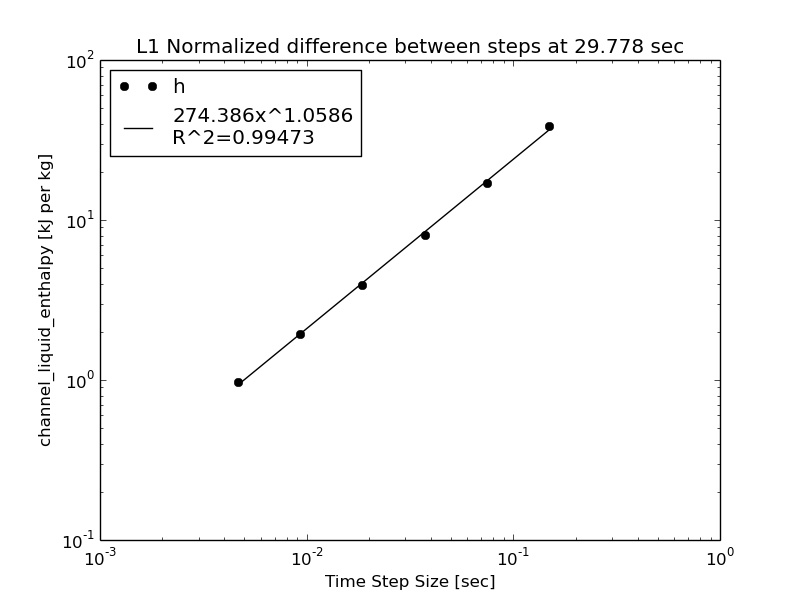
\includegraphics[width=0.50\textwidth]{images/Isokinetic_Advection/Difference_h}
%    	\caption{Scaling of numerical error with constant time step size for
%    	enthalpy}
%    	\label{fig:Difference_h}
%    \end{figure}
    
    
    \begin{figure}[!h]
    	\centering
    	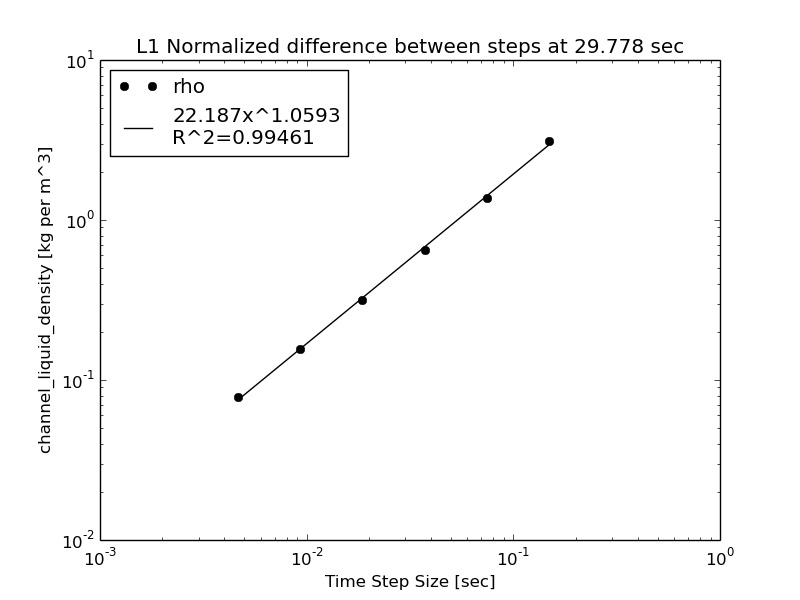
\includegraphics[width=0.50\textwidth]{images/Isokinetic_Advection/Difference_rho}
    	\caption{Scaling of numerical error with constant time step size for
    	density}
    	\label{fig:Difference_rho}
    \end{figure}
    
    The power fit for density has a high correlation coefficient, and
    shows that the order of accuracy temporally is close to 1. Richardson
    extrapolation to determine the order of accuracy at each point as shown by 
    figure \ref{fig:Temporal_Order_Of_Accuracy_rho}. As the time step size
    decreases, the order of accuracy approaches 1.0 due to smaller higher order
    terms. 
        
%   \begin{figure}[!h]
%   	\centering
%   	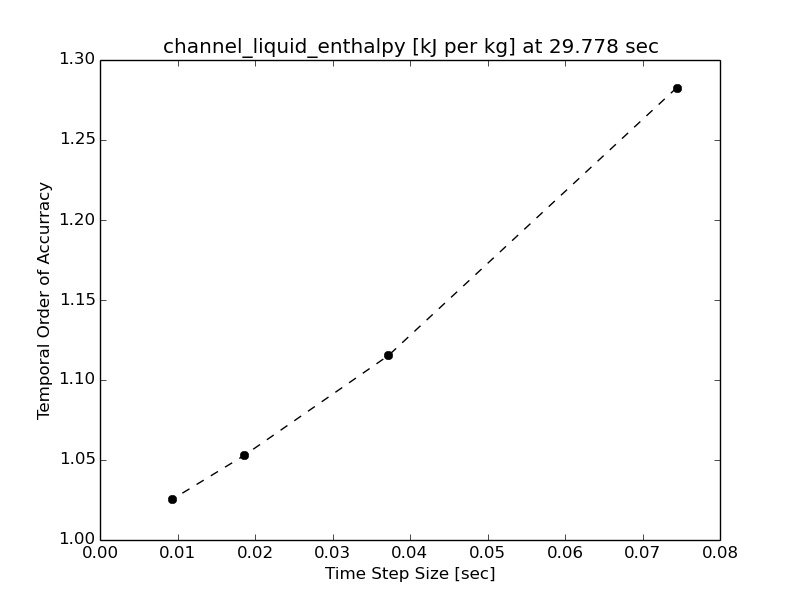
\includegraphics[width=0.50\textwidth]{images/Isokinetic_Advection/Temoral_Order_Of_Accuracy_h}
%   	\caption{Temporal Order of Accuracy for density}
%   	\label{fig:Temporal_Order_Of_Accuracy_h}
%   \end{figure}
    
    \begin{figure}[!h]
    	\centering
    	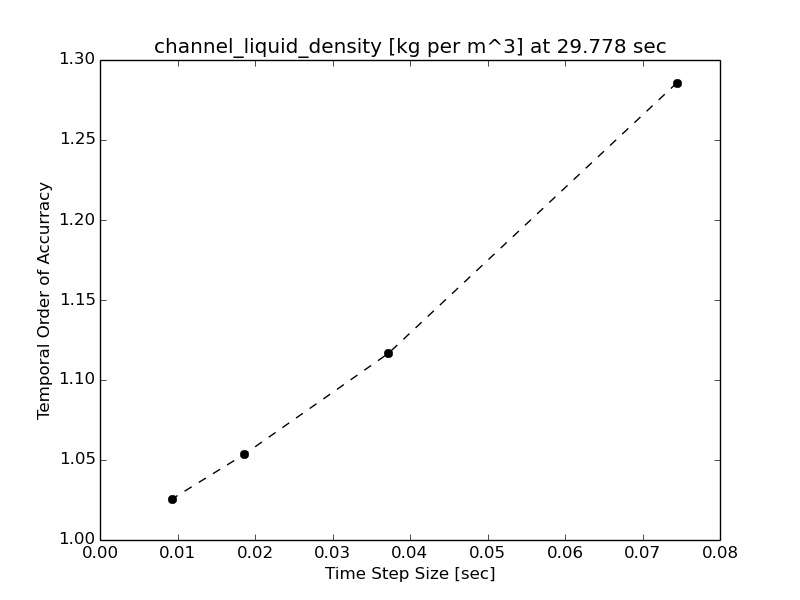
\includegraphics[width=0.50\textwidth]{images/Isokinetic_Advection/Temoral_Order_Of_Accuracy_rho}
    	\caption{Temporal Order of Accuracy for density}
    	\label{fig:Temporal_Order_Of_Accuracy_rho}
    \end{figure}
    
    When the CFL number is set to 1, the spatial error and temporal error
    cancel out producing a perfect square wave in time and space as shown by
    figure \ref{fig:density_2D}. This holds true for a variety of spatial
    mesh sizes, confirming that both the temporal and spatial errors are first
    order accurate. 
    
    \begin{figure}[!h]
    	\centering
    	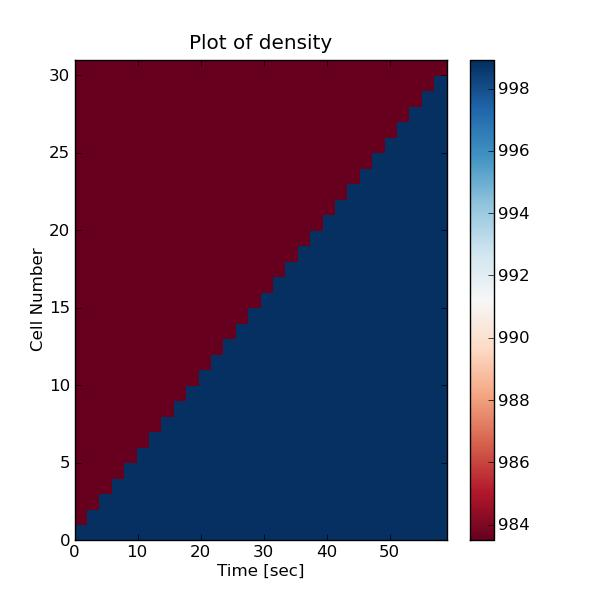
\includegraphics[width=0.50\textwidth]{images/Isokinetic_Advection/density_2D}
    	\caption{Advection of isokinetic density wave $\frac{kg}{m^{3}}$ in time
    	and space for CFL=1}
    	\label{fig:density_2D}
    \end{figure}








